\documentclass[a4paper,12pt]{article}


\usepackage{setspace}
\usepackage{xcolor}
\usepackage{graphicx}
\usepackage{geometry}
\usepackage{float}
\usepackage{titlesec}
\usepackage{subfigure}
\usepackage{caption}
\captionsetup{figurewithin=section}
\usepackage{amsmath}
\usepackage{enumitem}
\usepackage{amssymb}
\usepackage{mathrsfs}

\begin{document}

\title{\textbf{Homework 5}}
\author{Yunian Pan}
\maketitle{}

\section{Problem 1: Bayesian Network Conditional Independence}

\begin{figure}[htp]
\centering
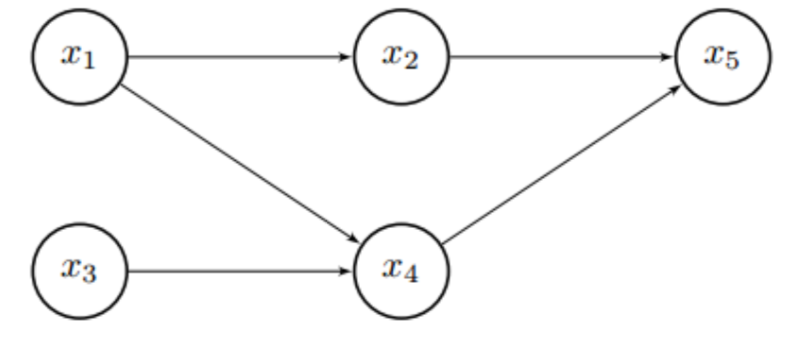
\includegraphics[width = .8\textwidth]{/Users/union/Desktop/fig1.png}
\end{figure}
 Below is the factorization of the probability distribution $p(x_1, \ldots, x_5) $implied by this directed graph:
\begin{align}
 p(x_1, \ldots, x_5) = p(x_1)p(x_3)p(x_2\lvert x_1)p(x_4 \lvert x_1,x_3)p(x_5 \lvert x_2, x_4) \nonumber
\end{align}

Using the Bayes ball algorithm, the statements
\begin{enumerate}
\item $x_2$ and $x_4$ are independent. 

False, the path going through between $x_2$ and $x_4$ is  $x_2 \to x_1 \to x_4$.

\item $x_2$ and $x_4$ are conditionally independent given $x_1$, $x_3$, and $x_5$.

False, the path going through between $x_2$ and $x_4$ is $x_2 \to x_5 \to x_4$.

\item $x_2$ and $x_4$ are conditionally independent given $x_1$, $x_3$.

True, there's no path going through between $x_2$ and $x_4$ given $x_1$, $x_3$.

\item $x_5$ and $x_3$ are conditionally independent given $x_4$,

False, the path is $x_5 \to x_2 \to x_1 \to x_4 \to x_3$.

\item $x_5$ and $x_3$ are conditionally independent given $x_1$, $x_2$, and $x_4$.

True, there's no path going through between $x_5$ and $x_3$ given $x_1$, $x_2$ and $x_4$.

\item $x_1$ and $x_3$ are conditionally independent given $x_5$.

False, the path is $x_1 \to x_2 \to x_5 \to x_4 \to x_3$.

\item $x_1$ and $x_3$ are conditionally independent given $x_2$.

True, there's no path going through between $x_1$ and $x_3$ given $x_2$.

\item $x_2$ and $x_3$ are independent.

True, there's no path going through between $x_1$ and $x_3$.

\item $x_2$ and $x_3$ are conditionally independent given $x_5$.

False, the path is $x_2 \to x_5 \to x_4 \to x_3$.

\item $x_1$ and $x_3$ are conditionally independent given $x_5$ and $x_4$.

False, the path is $x_2 \to x_1 \to x_4 \to x_3$.

\end{enumerate}


\section{Problem 2:  Junction Tree}

\begin{figure}[hbp]
\centering
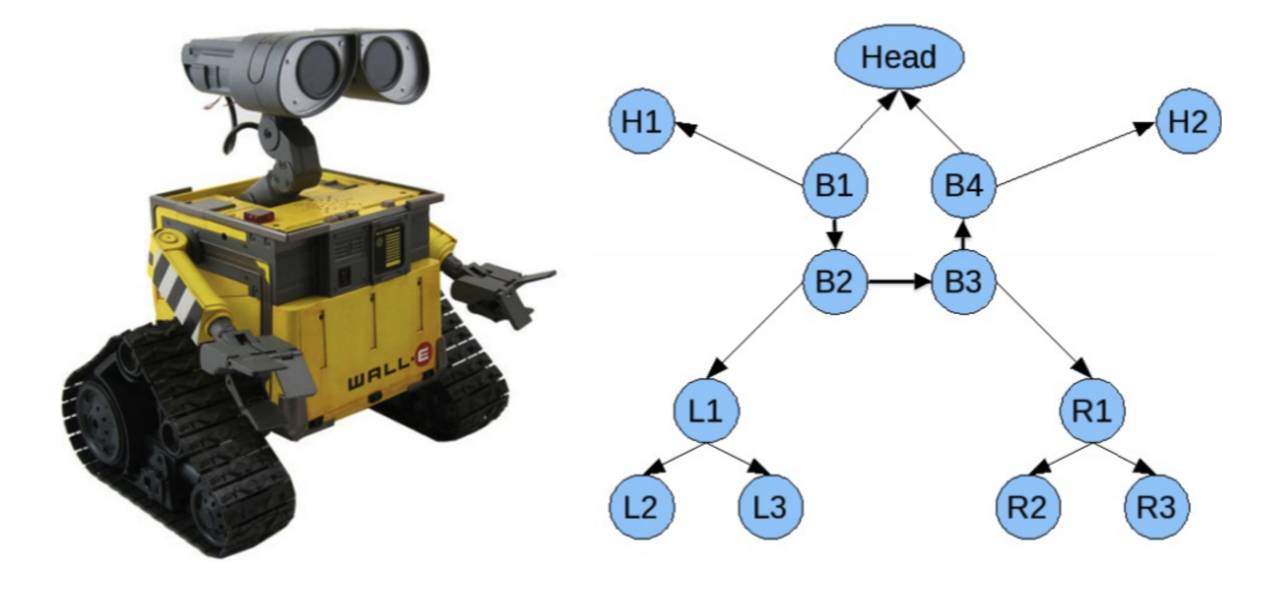
\includegraphics[width = .8\textwidth]{../../../../Desktop/eve.png}
\end{figure}

After moralization and triangulation:
\begin{figure}[htp]
\subfigure[moralization]{
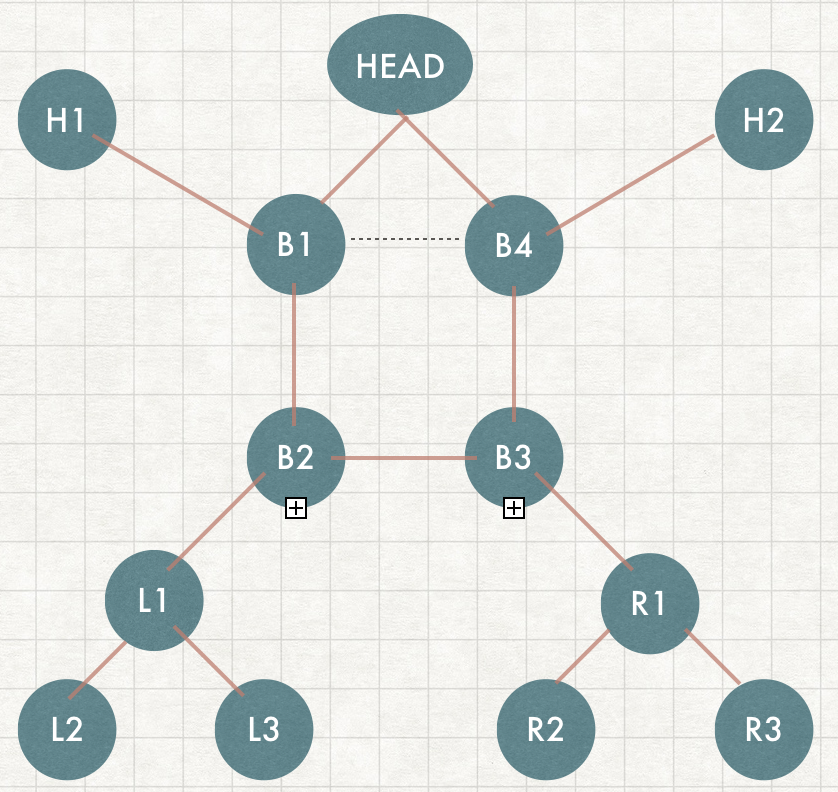
\includegraphics[width = .49\textwidth]{../../../../Desktop/moralization.png}}
\subfigure[triangulation]{
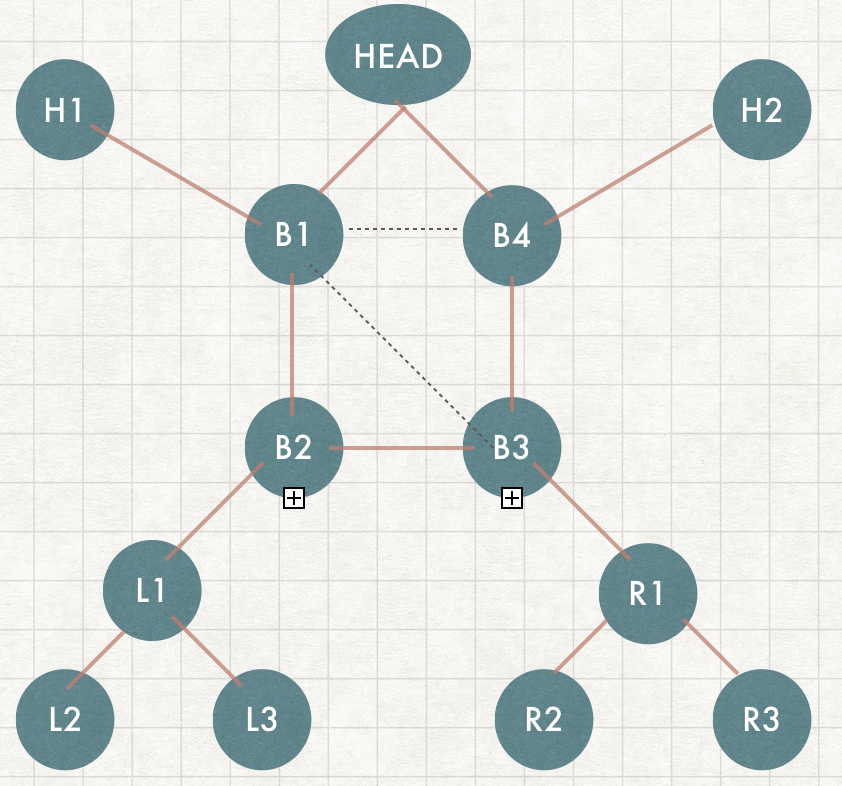
\includegraphics[width = .49\textwidth]{../../../../Desktop/triangulation.png}}
\end{figure}

Build a junction tree:
\begin{figure}[htp]
\subfigure[find cycle]{
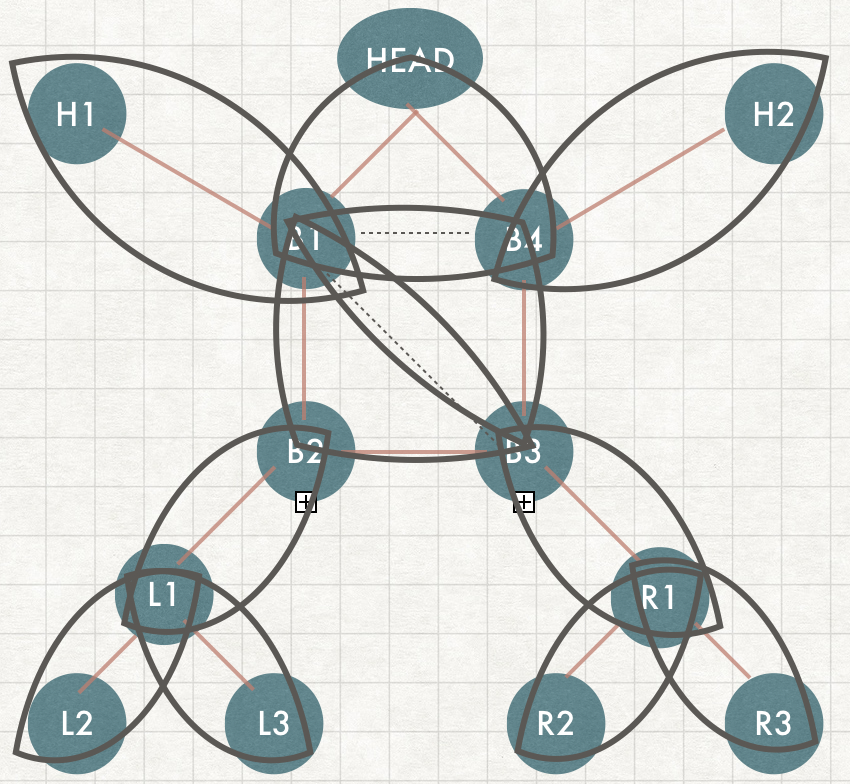
\includegraphics[width = .49\textwidth]{../../../../Desktop/clique.png}}
\subfigure[junction tree]{
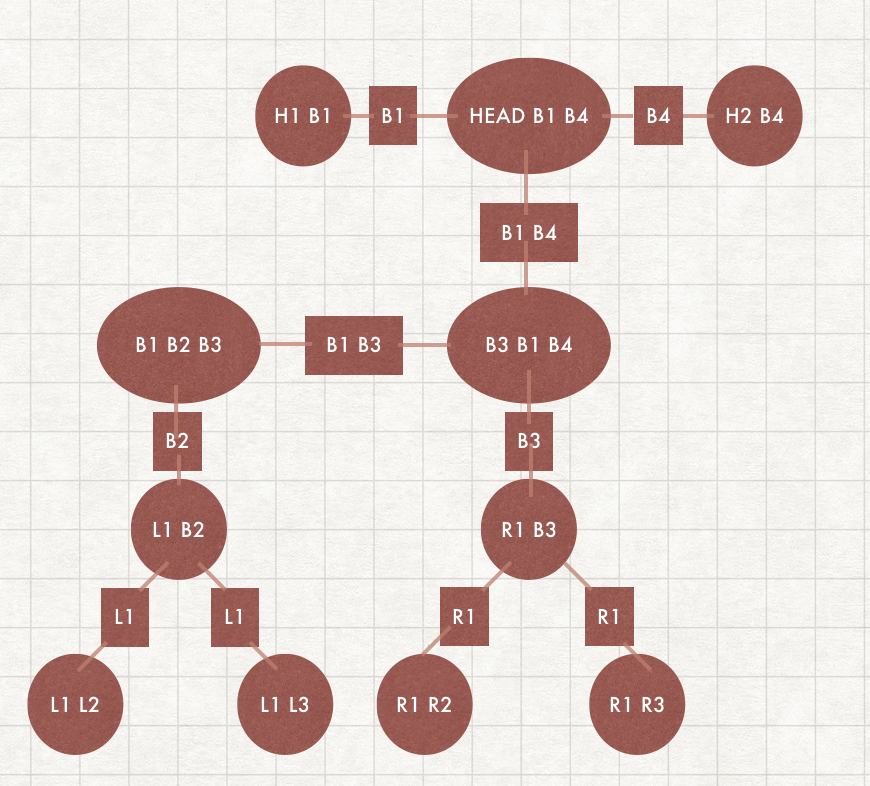
\includegraphics[width = .51\textwidth]{../../../../Desktop/junctiontree.png}}
\end{figure}



\section{Problem 3: Neural Networks}

For dataset 1, I consider it to be mapped to a linearly separable set whose features are the norms of each data point $X_1^2+X_2^2$, so the simplest way is to design a single neuron, it can be a SVM or a perceptron or whatever, as shown in $\ref{d1}$, I use the ReLu function with no regularization, feed in the $X_1^2$ and $X_2^2$ properties, it can be done with test loss and training loss both being 0.001.
\begin{figure}[hp]
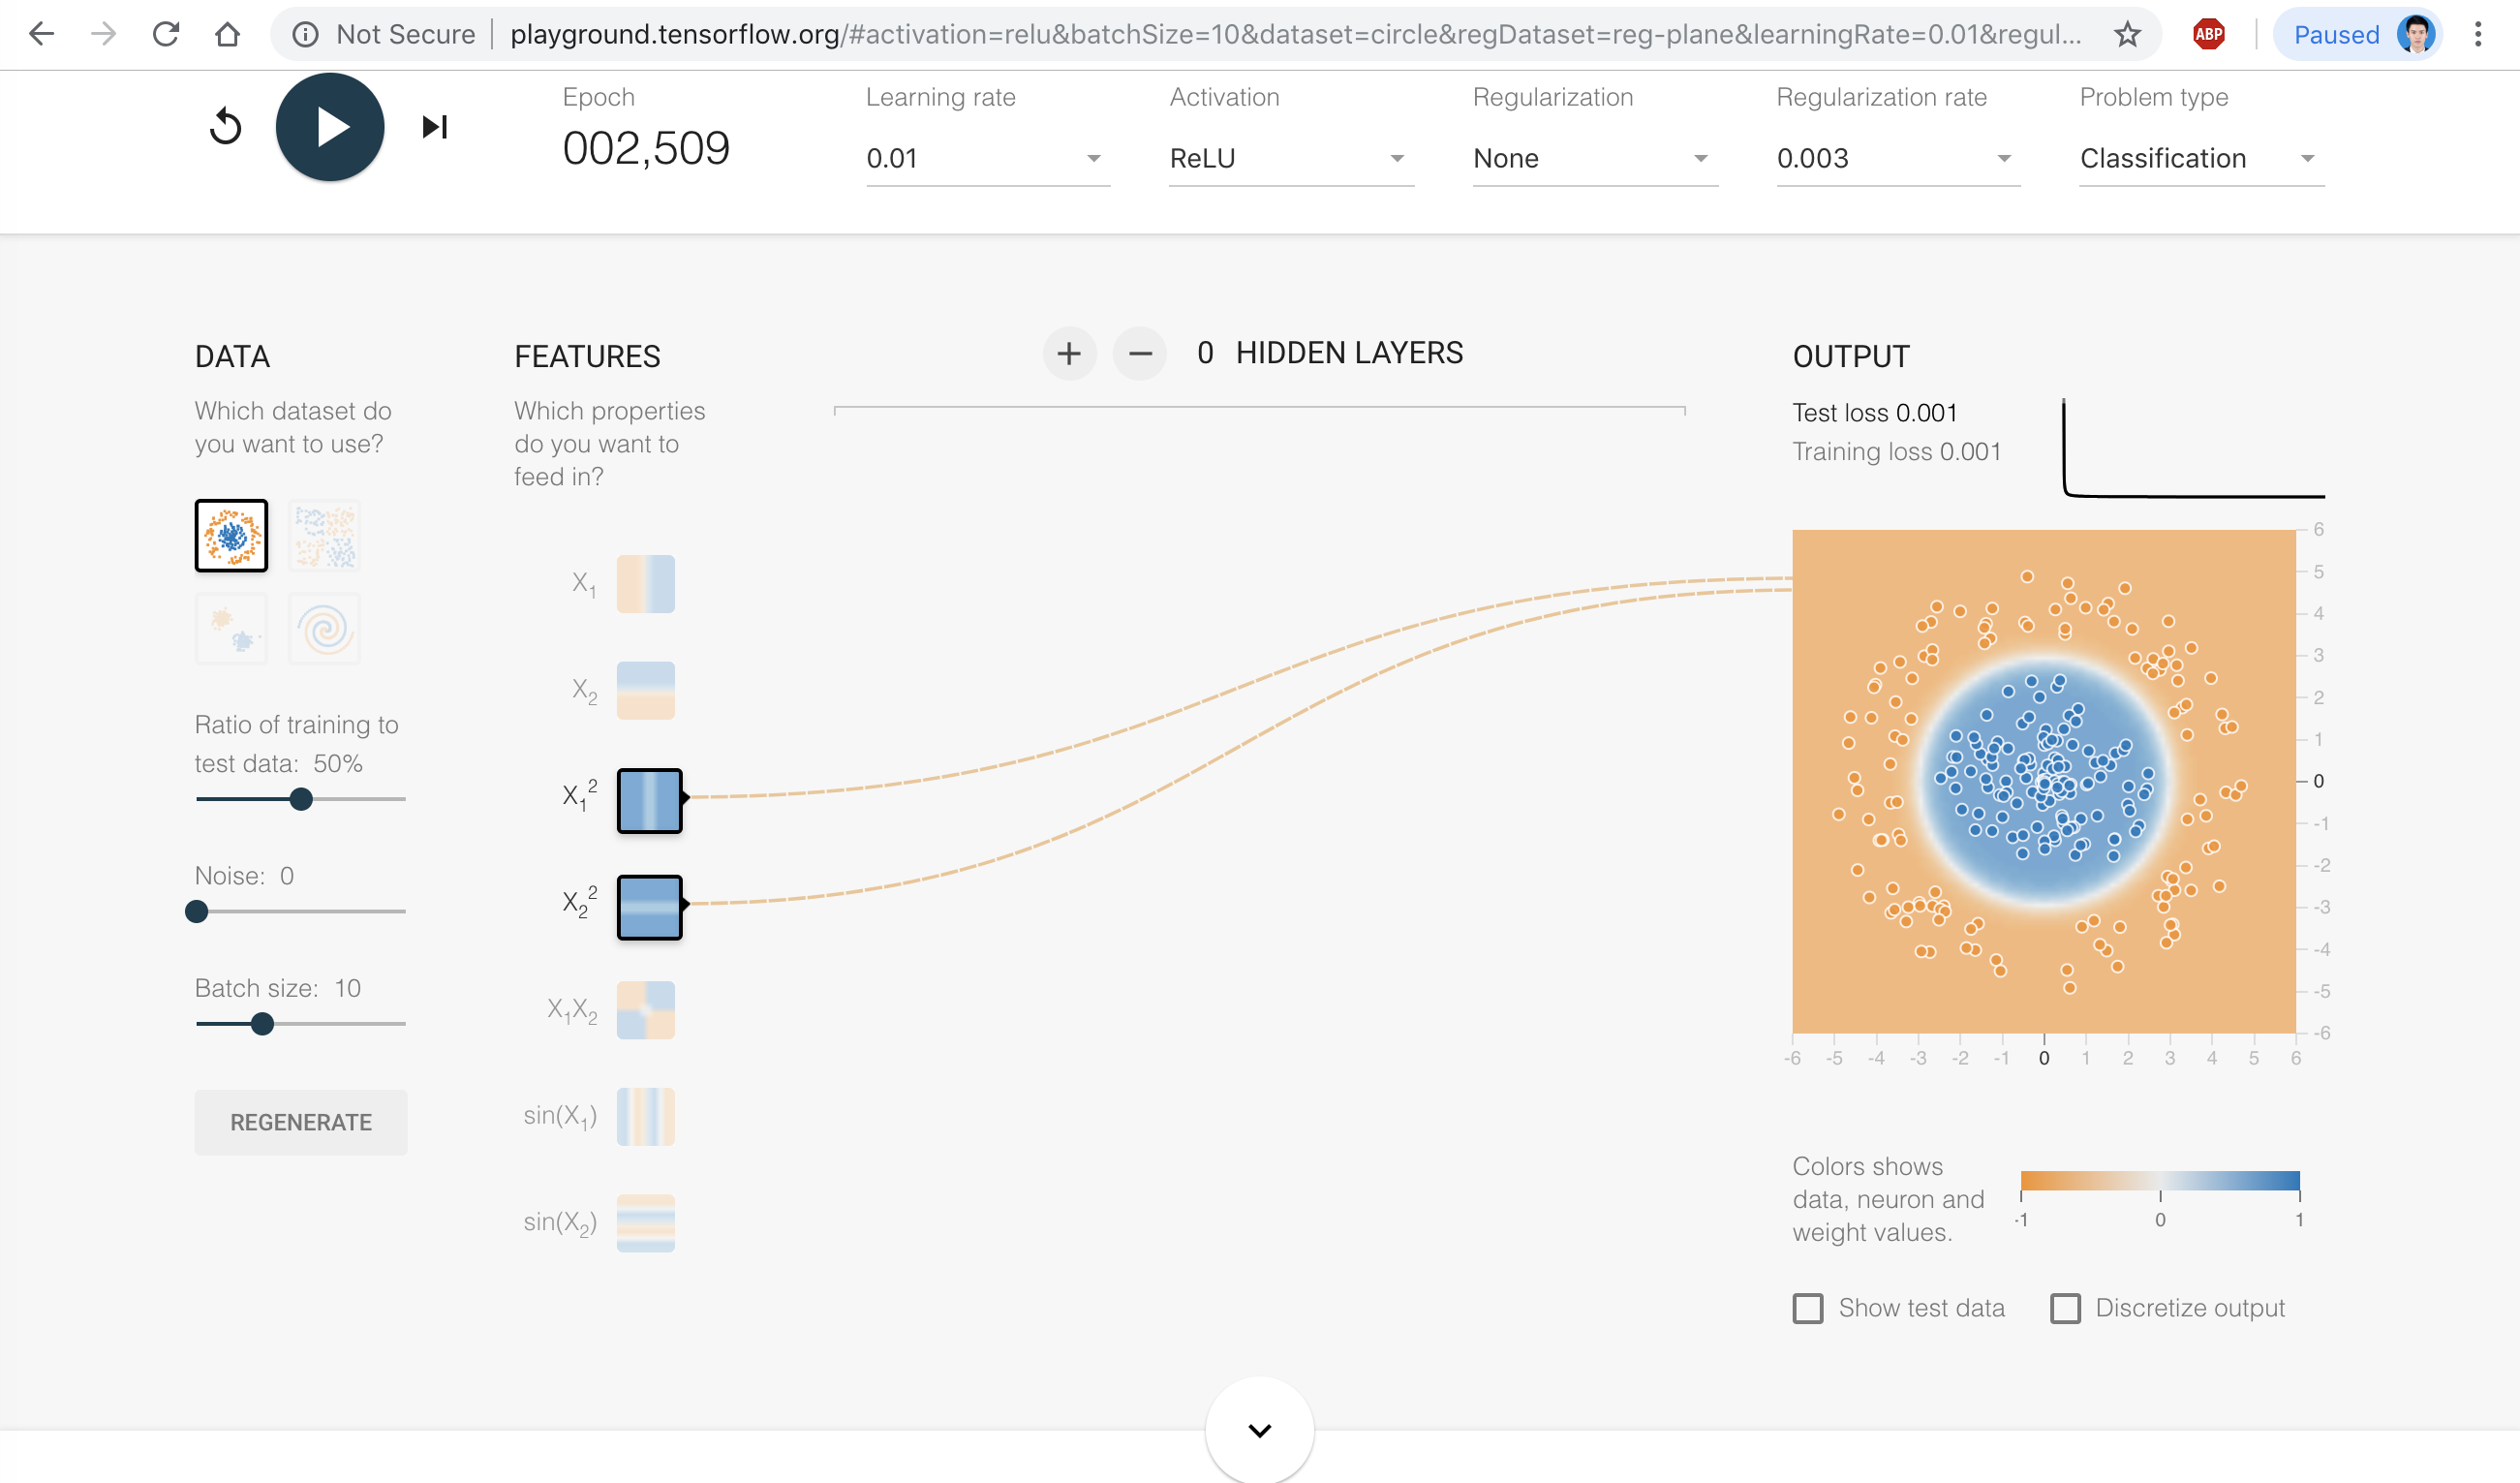
\includegraphics[width = \textwidth]{../../../../Desktop/d1.png}}
\caption{dataset 1}
\label{d1}
\end{figure}
But with a hidden layer and linear activate function as shown in $\ref{d12}$ the test loss and training loss both reached 0 after 1300 epochs, which means no overfitting.
\begin{figure}[hp]
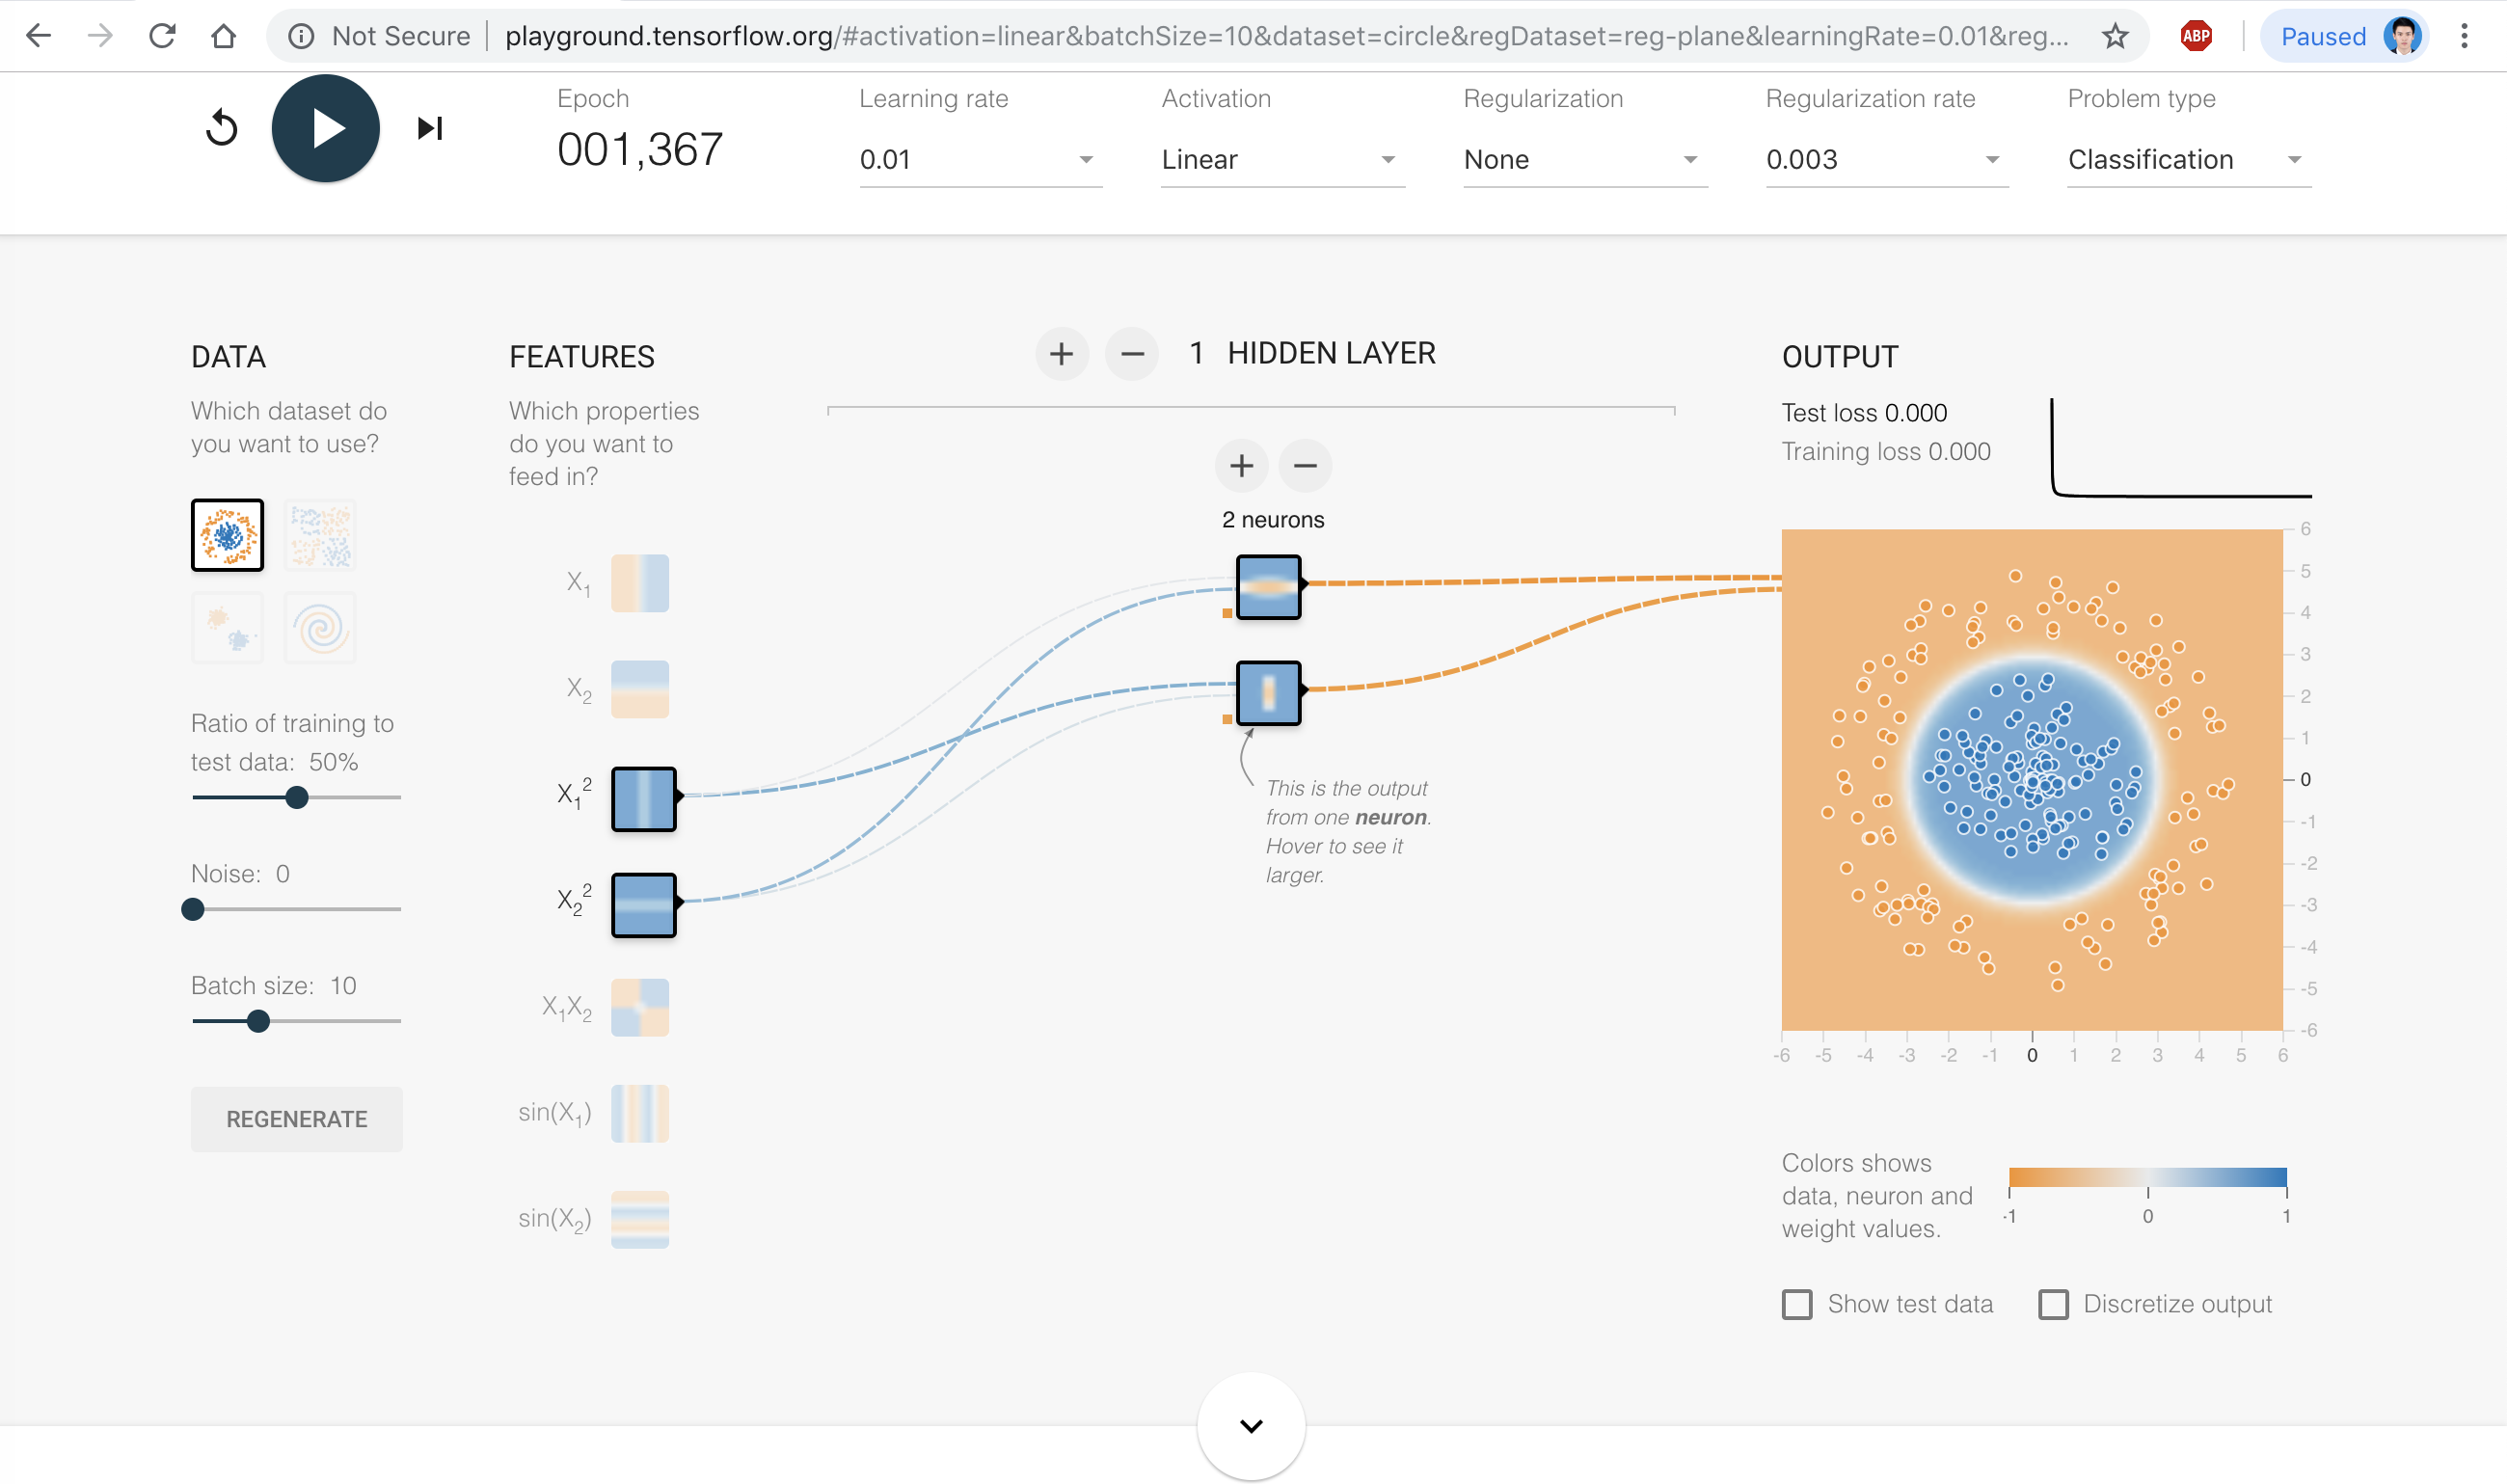
\includegraphics[width = \textwidth]{../../../../Desktop/d1(2).png}}
\caption{dataset 1(2)}
\label{d12}
\end{figure}

For dataset 2, we can use a sign classifier to separate $X_1X_2>0$ and $X_1X_2<0$, therefore I use the ReLu function again as a single neuron to establish the classifier, as shown in $\ref{d2}$.
\begin{figure}[hp]
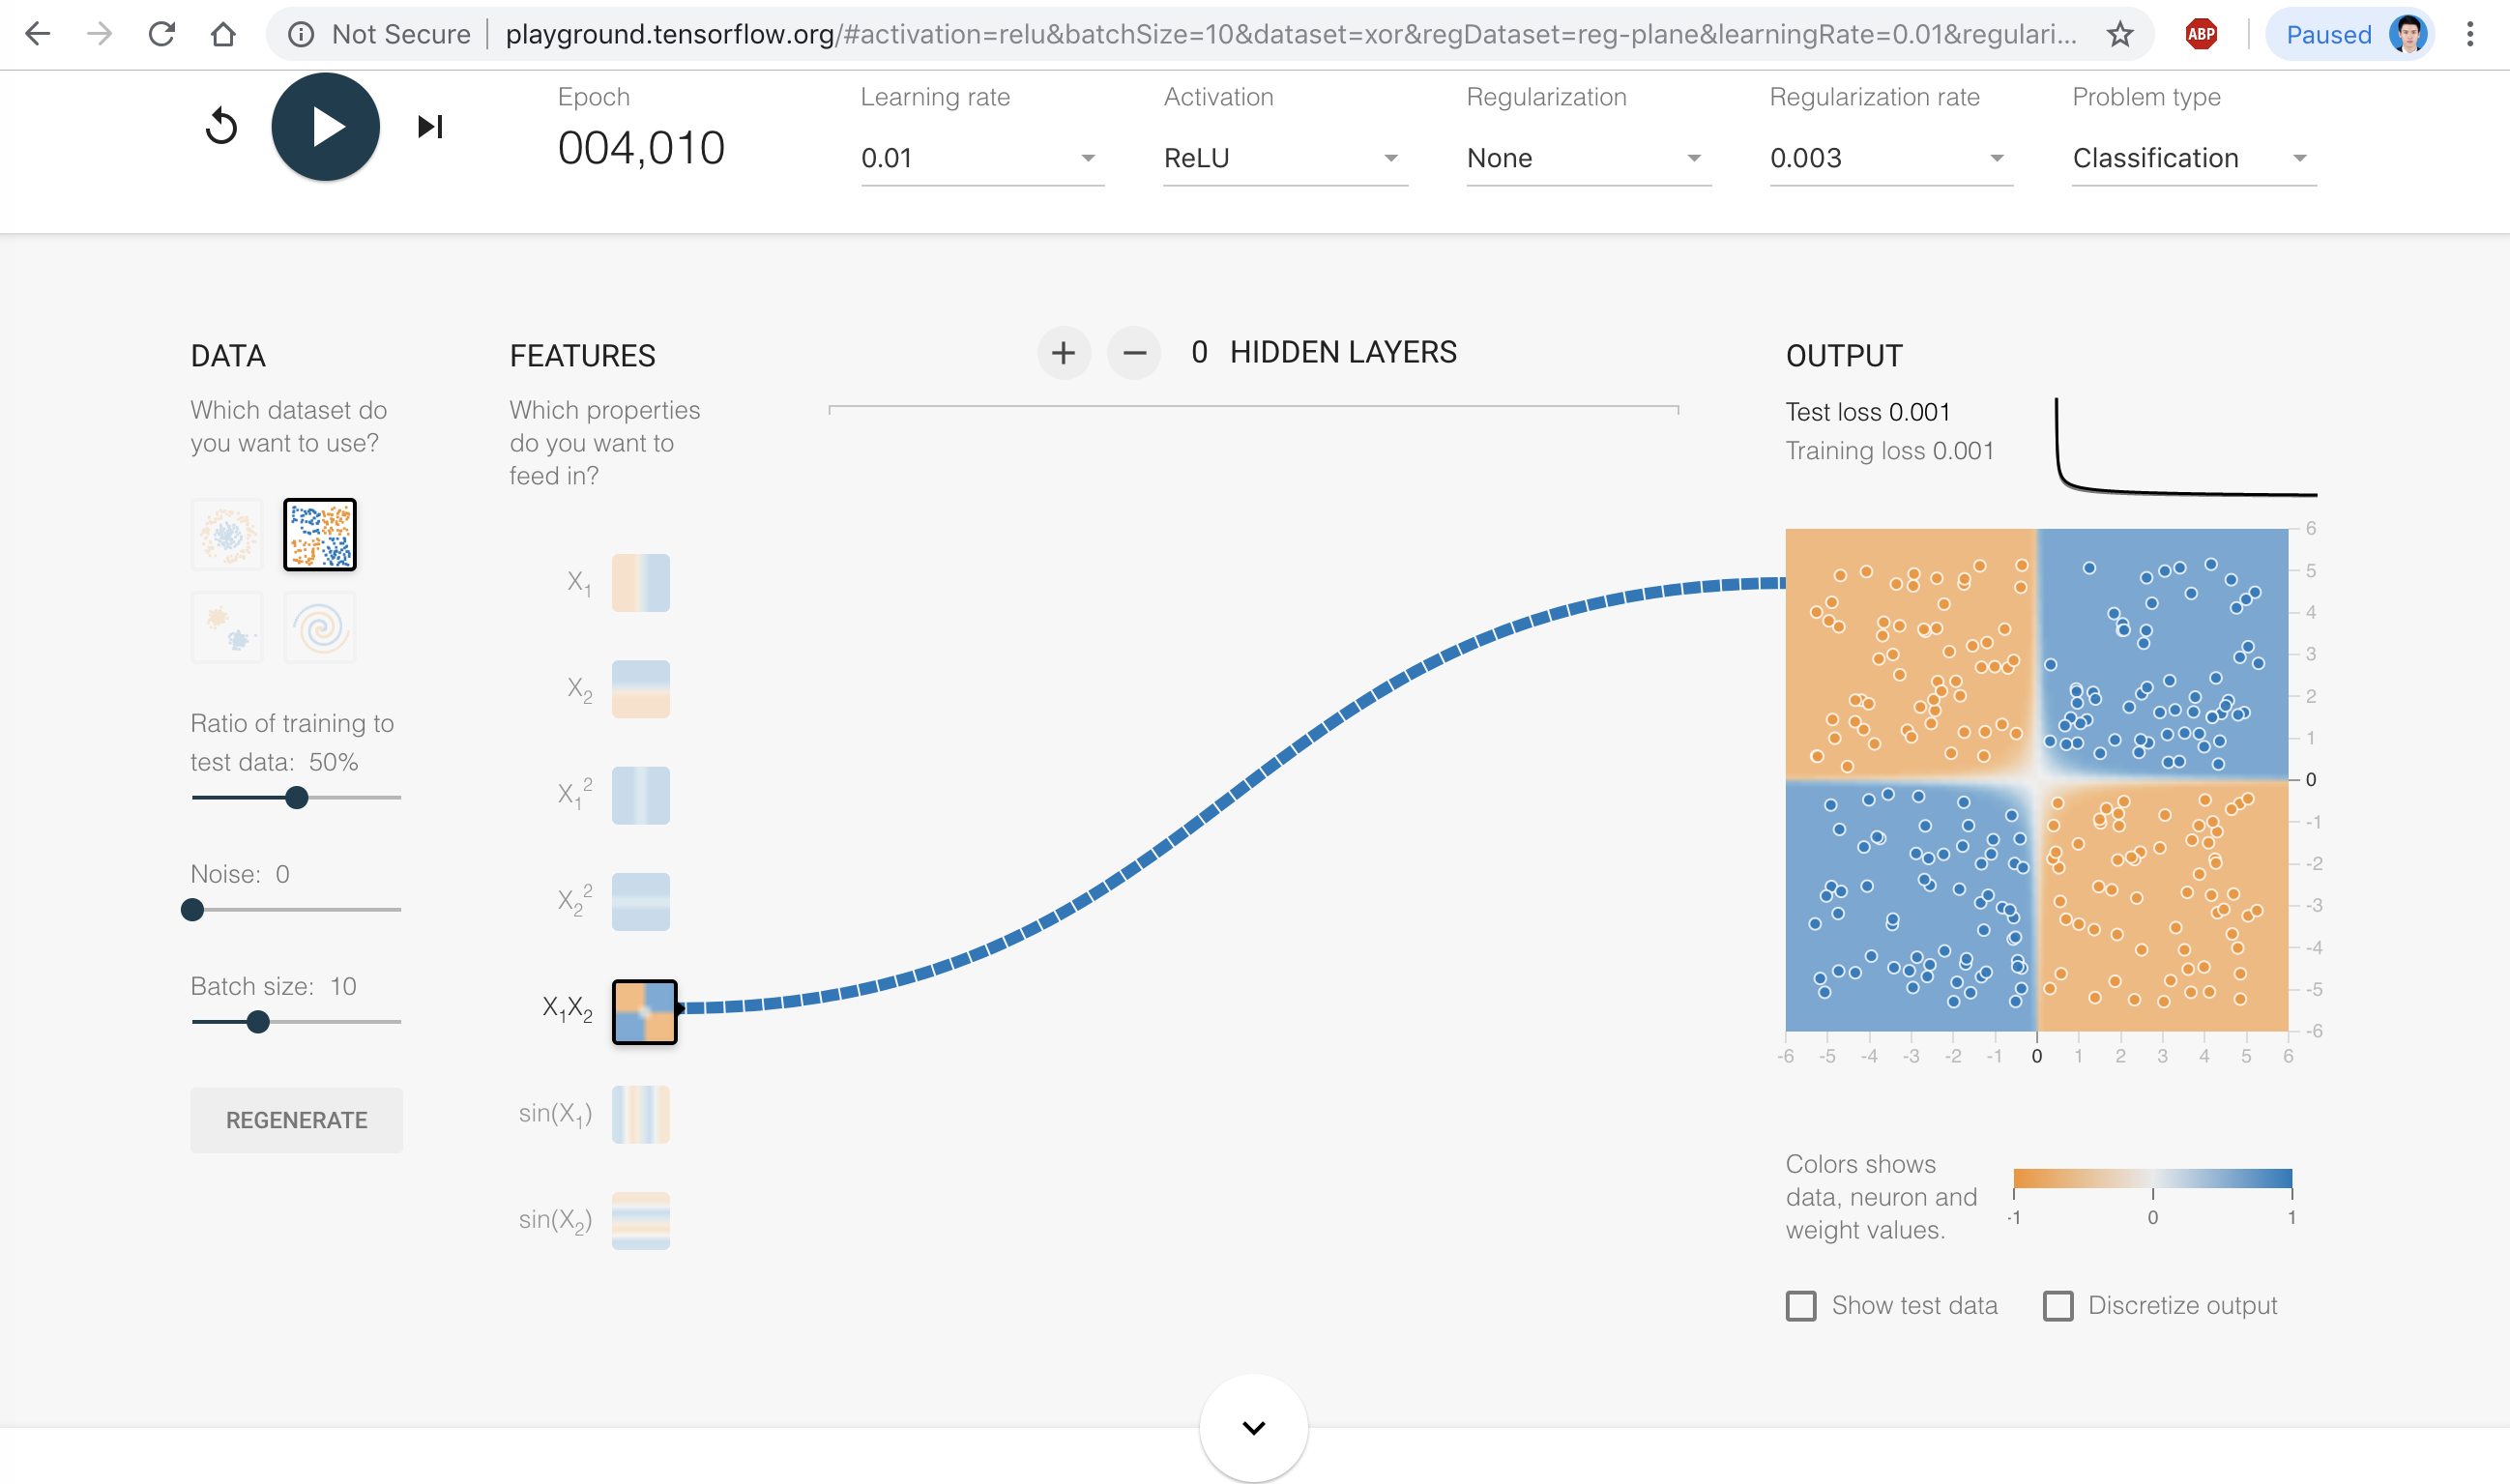
\includegraphics[width = \textwidth]{../../../../Desktop/d2.png}}
\caption{dataset 2}
\label{d2}
\end{figure}

For dataset 3, the data points are similar to 2 different 2D-Gaussian distributions with 2 different centers, so I add a hidden layer and a $L_2$ regularization to model the properties of the data set, as shown in $\ref{d3}$.
\begin{figure}[hp]
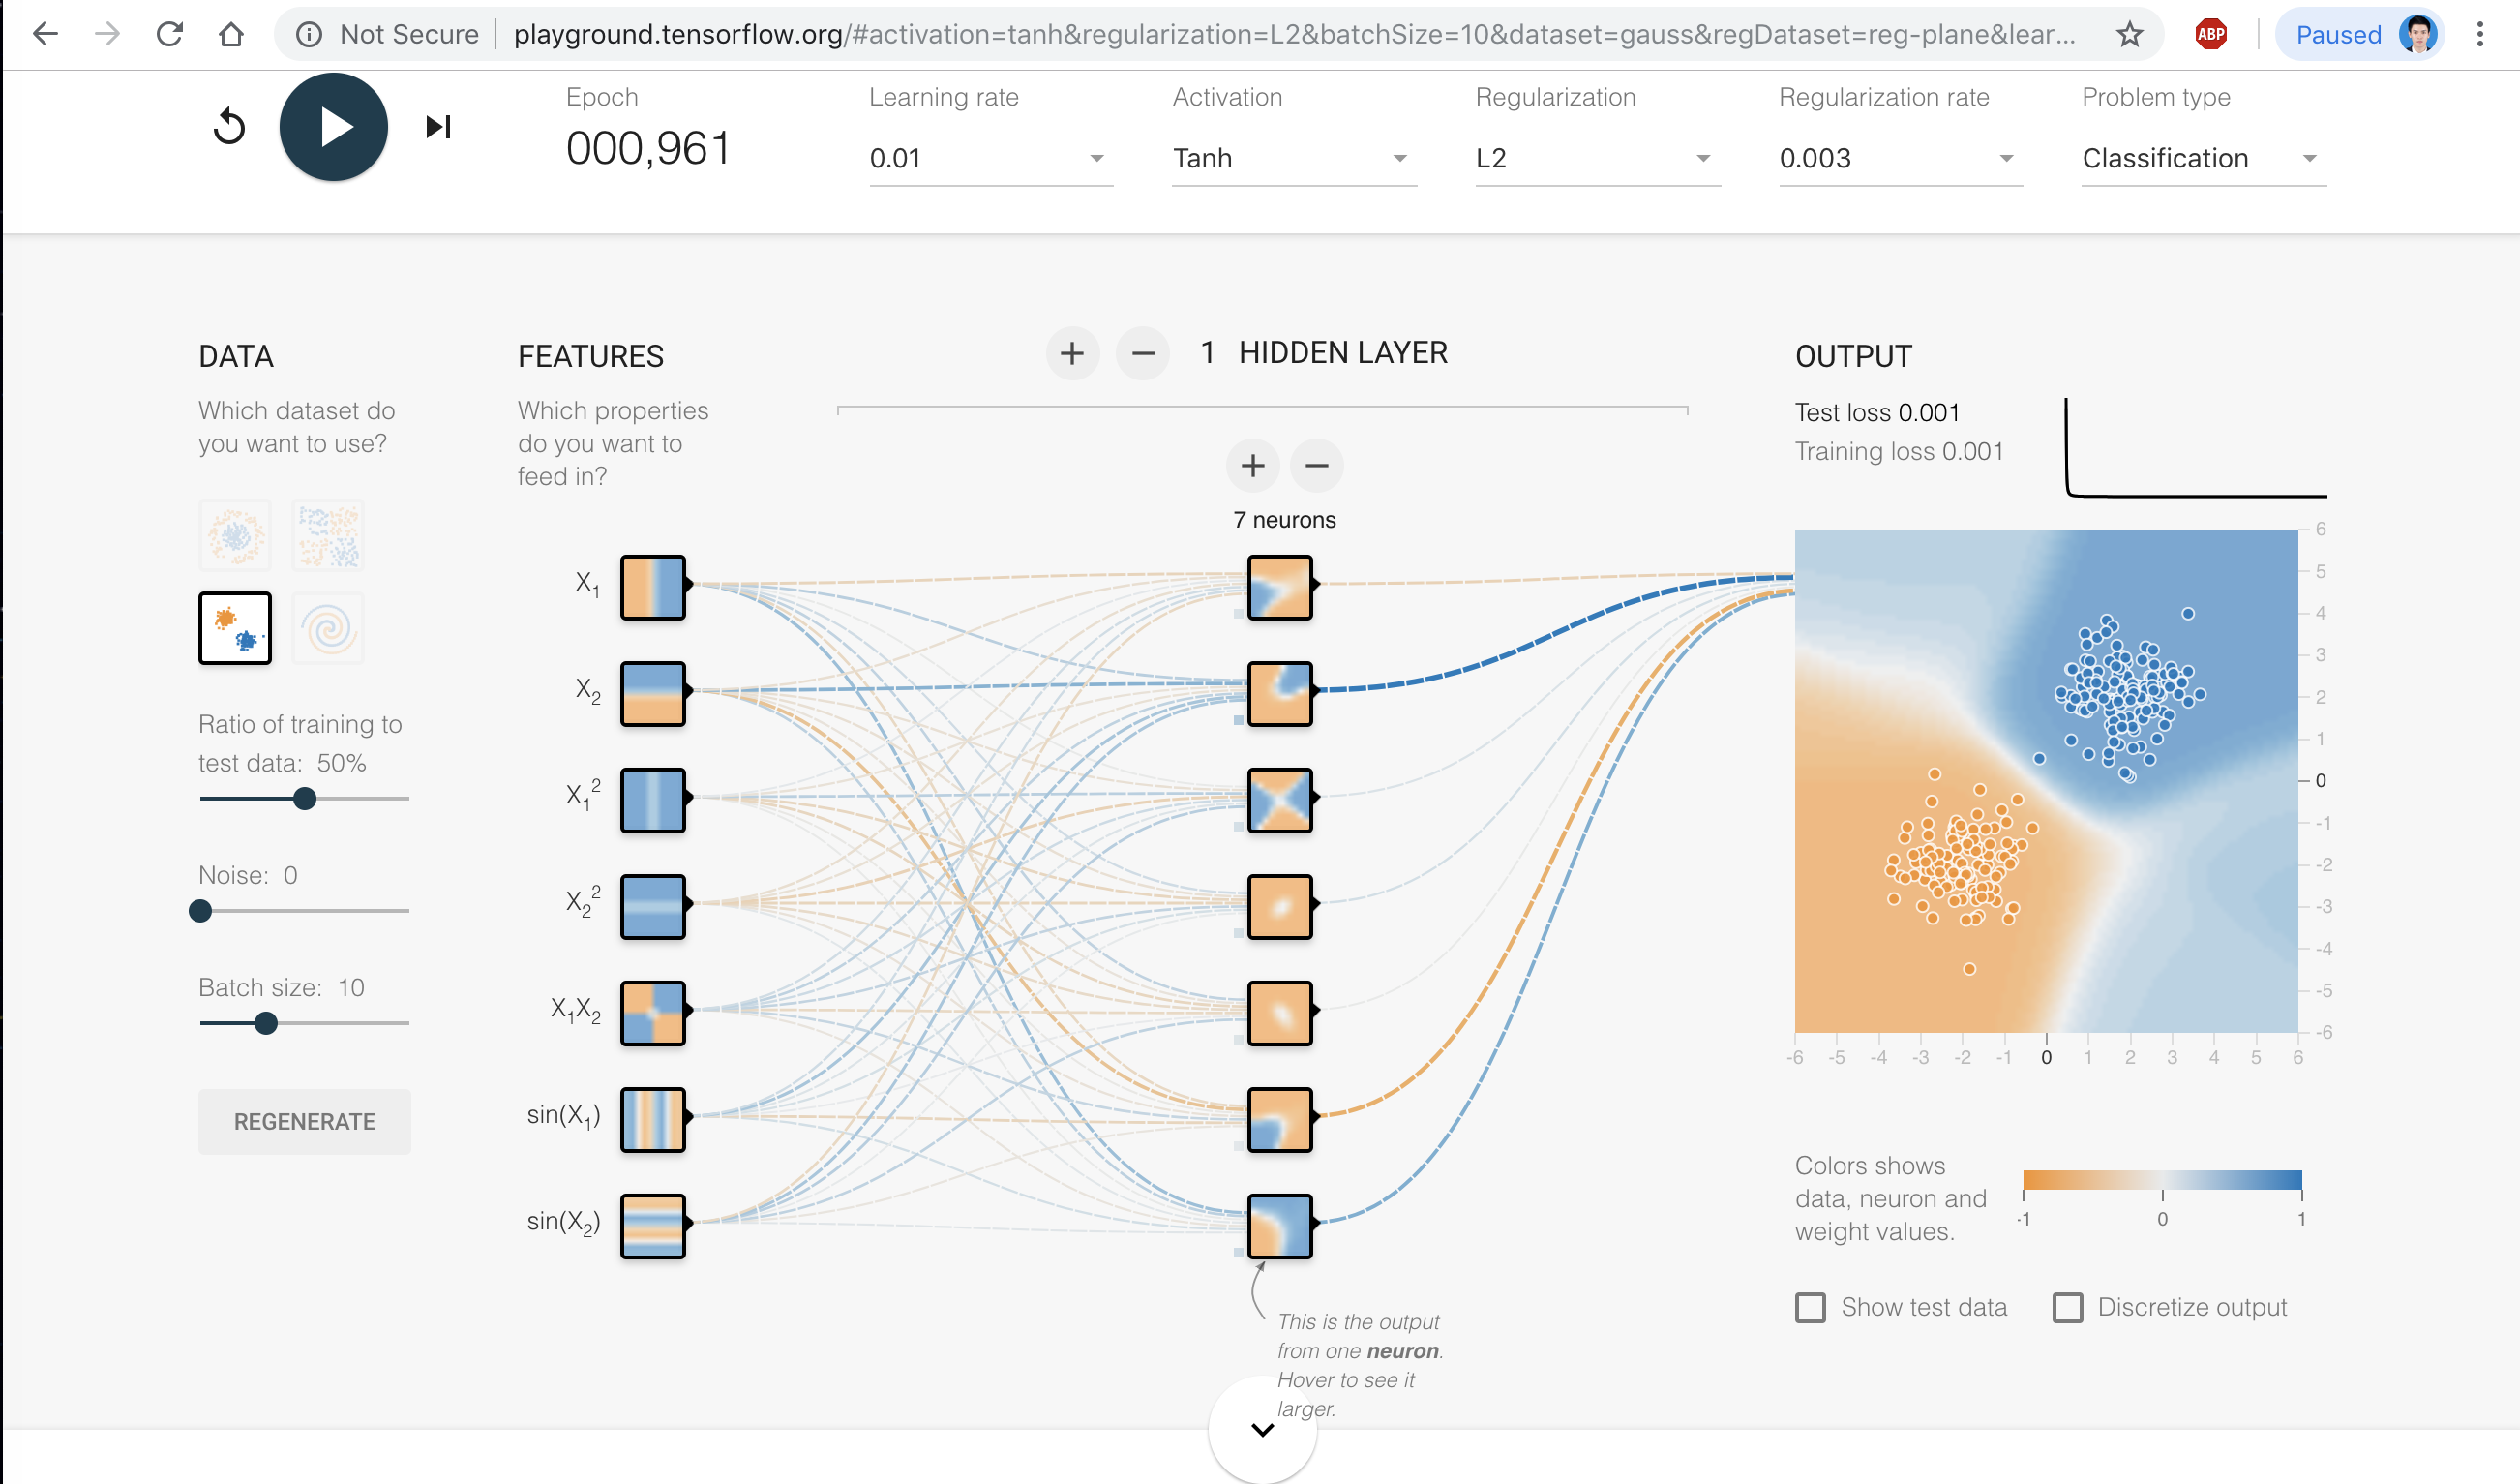
\includegraphics[width = \textwidth]{../../../../Desktop/d3.png}}
\caption{dataset 3}
\label{d3}
\end{figure}

For dataset 4, it's not possible to design an extremely simple network to classify such a double helix data set,  2 hidden layers are used, along with $L_2$ regularization in case of overfitting and tahn activate function, as shown in $\ref{d4}$
\begin{figure}[hp]
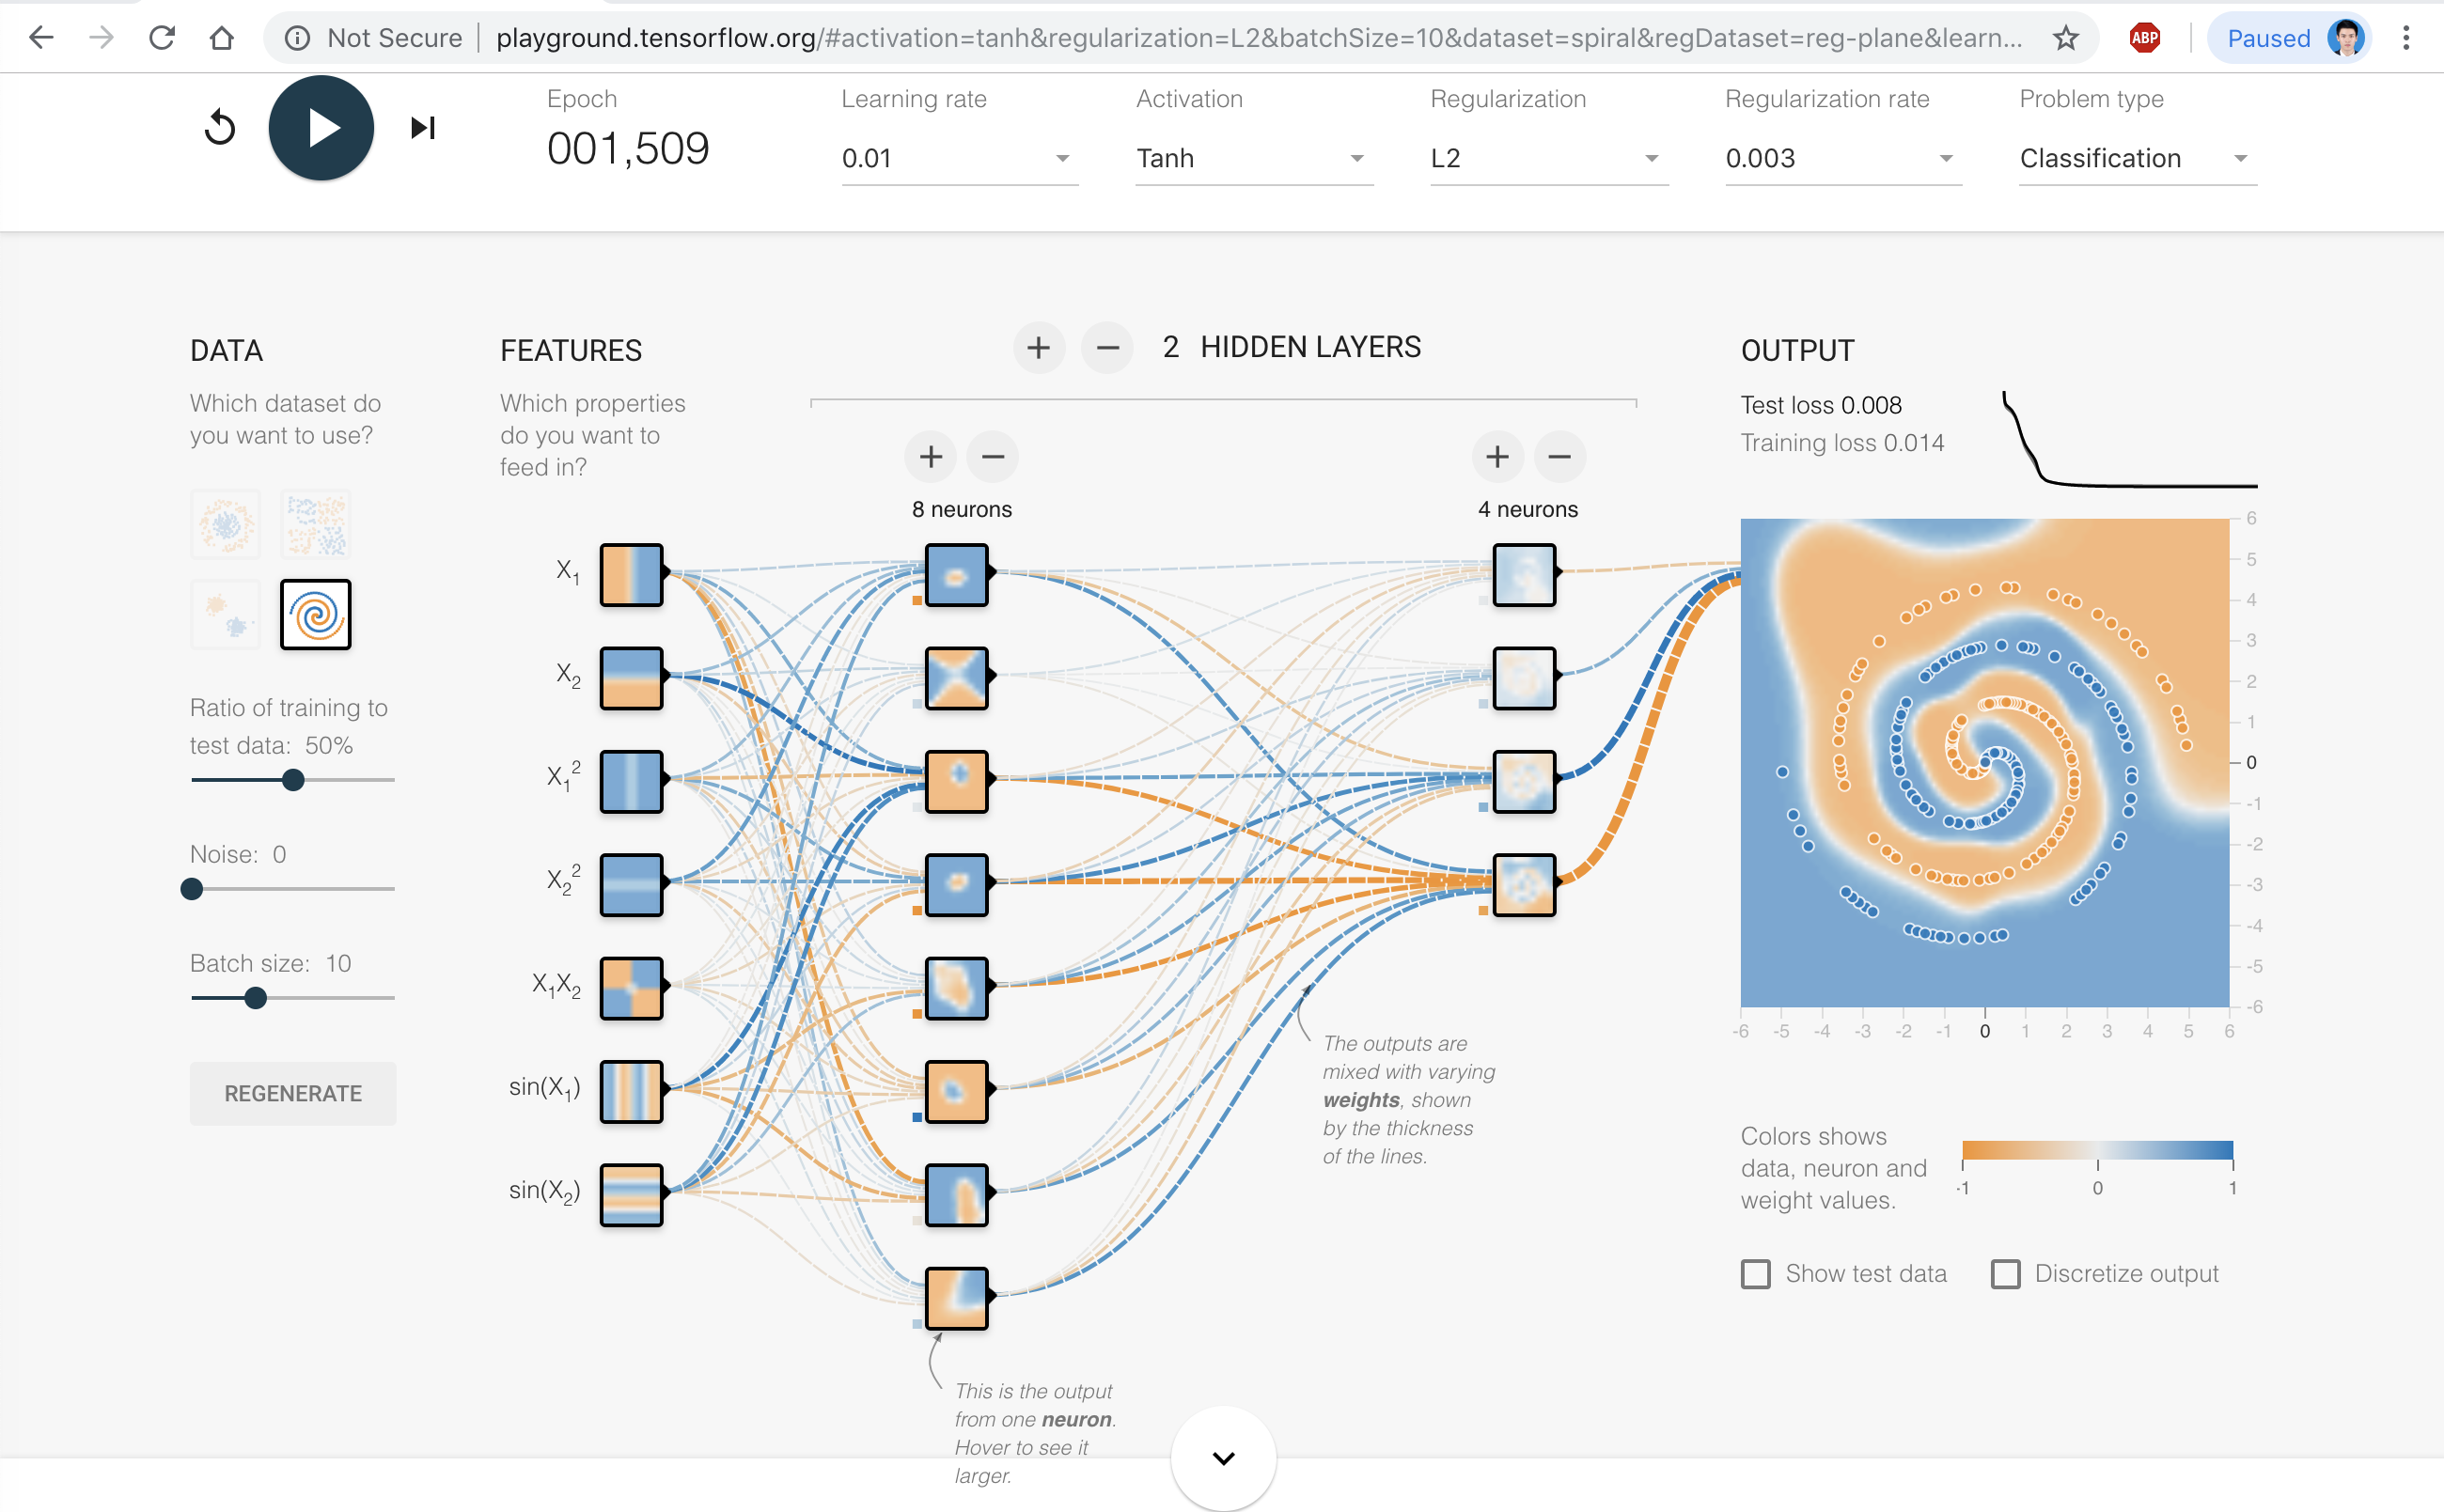
\includegraphics[width = \textwidth]{../../../../Desktop/d4.png}}
\caption{dataset 4}
\label{d4}
\end{figure}


\end{document}


